\section{Data}

We are given the evaluation data from a previous offering of this course. Our first step was to explore the data, for instance :

\begin{itemize}
    \item What type of attributes are present?
    \item How are the attributes distributed?
    \item How does attendance affect the grade?
\end{itemize}


We observe that in total, there are \textbf{500} examples in the dataset. This is a \textbf{classification} task, where we predict the student's \textbf{grade}, which takes $8$ values, in $\{\text{A , A- , B , B- , C , C- , D , E}\}$. \\

\begin{tabular}{ |p{3cm}||p{3cm}|p{5cm}|}
\hline
\multicolumn{3}{|c|}{Attribute Description}\\
\hline
Attribute& Type &  Classes {discrete} \\
 & & Range (continuous)\\
\hline
Lab-Test1  &  Continuous& 0 - 30  \\
Lab-Test2 & Continuous  & 0 - 24 \\
Midsem Test & Continuous& 0 - 90\\
Gender    &Discrete & $\{\text{Male , Female}\}$\\
Attendance& Ordinal & $\{ \text{Low  ,  Moderate , High}\}$\\
\hline
\end{tabular}\newline \newline


When we split the dataset using the \textbf{70-30 rule}  into \textbf{training set} and \textbf{test set}, we get the following partition of data.\\


\begin{center}
\begin{tabular}{ |p{3cm}||p{5cm}|}
\hline
\multicolumn{2}{|c|}{Data split}\\
\hline
Set& Number of samples \\
\hline
Training &  350 \\
Test & 150 \\
\hline
\end{tabular}
\end{center} \\

Here are some exploratory visualisations for the given data:

\begin{figure}[htbp]
    \centering
    \begin{minipage}[b]{0.45\textwidth}
        \centering
        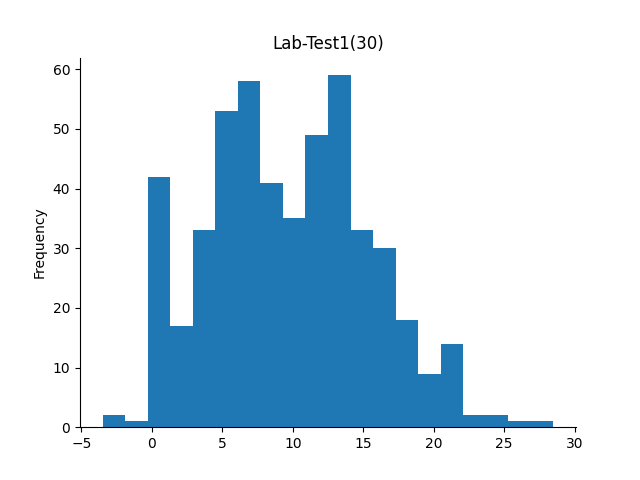
\includegraphics[width=\textwidth]{images/data_lab_test1.png}
        \caption*{Histogram: Lab Test 1 scores}
        \label{fig:image1}
    \end{minipage}
    \hfill
    \begin{minipage}[b]{0.45\textwidth}
        \centering
        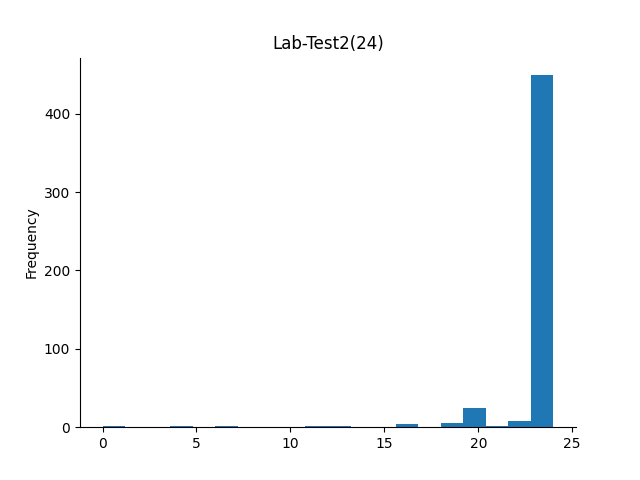
\includegraphics[width=\textwidth]{images/data_lab_test2.png}
        \caption*{Histogram: Lab Test 2 scores}
        \label{fig:image2}
    \end{minipage}
    \label{fig:overall}
\end{figure}

\begin{figure}[htbp]
    \centering
    \begin{minipage}[b]{0.45\textwidth}
        \centering
        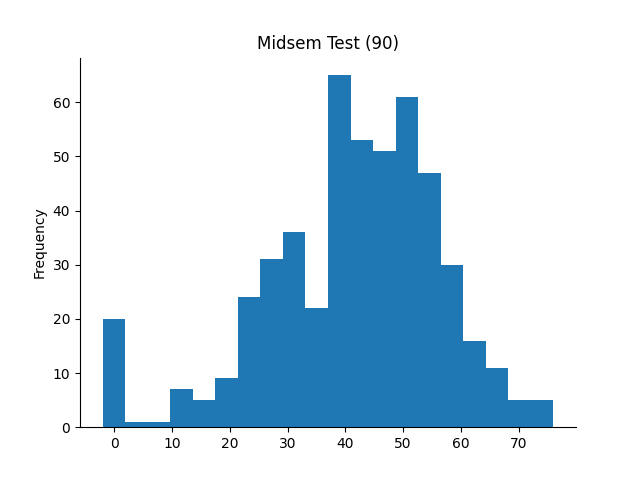
\includegraphics[width=\textwidth]{images/data_midsem.png}
        \caption*{Histogram: Mid-sem scores}
        \label{fig:image1}
    \end{minipage}
    \hfill
    \begin{minipage}[b]{0.45\textwidth}
        \centering
    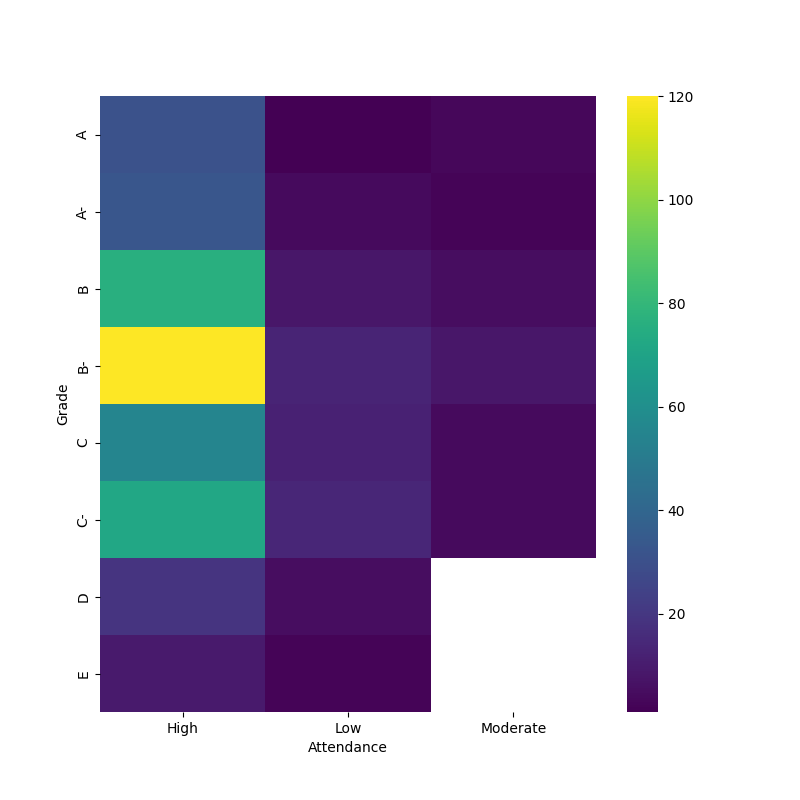
\includegraphics[width=\textwidth]{images/data_attendance_vs_grade.png}
        \caption*{Heatmap: Attendance vs Grade}
        \label{fig:image2}
    \end{minipage}
    \label{fig:overall}
\end{figure}

